% contient une explication du fonctionnement du Mip Map et du Rip Map, et des schémas explicatifs. En bref, un résumé de l'article de Williams
% parler éventuellement de la méthode naïve, ou d'autres méthodes actuelles qui ne fonctionnent pas



\ssse{Methode naive}

%petite explication de la méthode naive, puis :

\begin{figure}[h!]
\centering
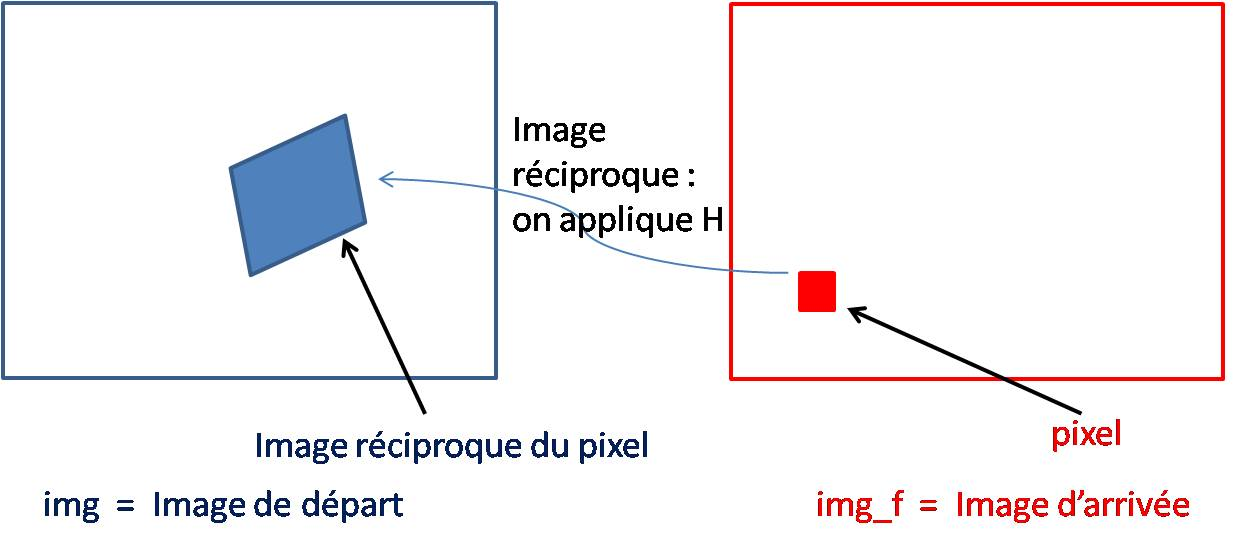
\includegraphics[scale=0.5]{imagereciproque.jpg}
\end{figure}

En pratique on utilise plutôt le Mipmap. C'est une méthode utilisée en texturing, présentée par Williams en 1983.

\ssse{Principe}

Le principe est de précalculer des coefficients qui représentent des zones entières de l'image, pour pouvoir ensuite calculer en temps réel une homographie. 

Pour cela on choisit de supposer que l'image est carrée de taille une puissance de 2 (quittes à faire un premier zoom). On calcul ensuite la valeur de certains carrés de l'image de taille une puissance de 2.
Le mipmap est donc représenté par une suite d'image chacune deux fois plus petite que la précédente, qui sont des "zoom-out" de l'image d'origine de facteur une puissance de 2.

%image d'un vrai mipmap, que je ferais moi
\begin{figure}[h!]
\centering
\caption{Un exemple de Mipmap}
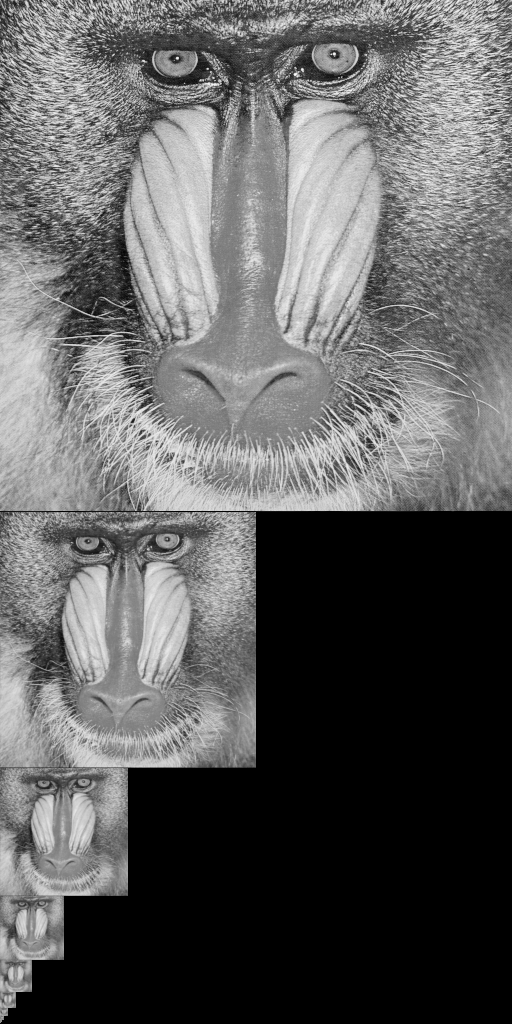
\includegraphics[scale=0.4]{MipMap_real}
\end{figure}

Ensuite, quand on cherche la valeur d'un pixel de l'image d'arrivée, on regarde la zone de l'image de départ à laquelle il correspond à l'aide des différentielles de l'homographie inverse. On obtient alors approximativement un parallélogramme, qu'on essaye d'approximer par des carrés.

%image de parallélogramme avec les différentielles, avec au mieux schéma image de départ / arrivé qui explique la correspondance entre un pixel est un parallélogramme

On appelle distance la taille d'un carré (car plus un pixel est "loin", plus les carrés qui l'approximent sont grands). 

On suppose une formule nous donnant la distance d'un point quelconque, la géométrie du mipmap ne permettant que des distances puissance de 2, on fait une approximation trilinéaire : 

-d'une part on fait une interpolation linéaire entre deux niveaux de profondeur qui encadrent la distance.

-d'autre part dans chaque niveau du mipmap on fait une interpolation bilinéaire entre les quatre carrés où tombe le pixel.

%image de l'inter trilinéaire avec deux plans pour les profondeurs
\begin{figure}[h!]
\centering
\caption{Schéma d'interpolation trilinéaire}
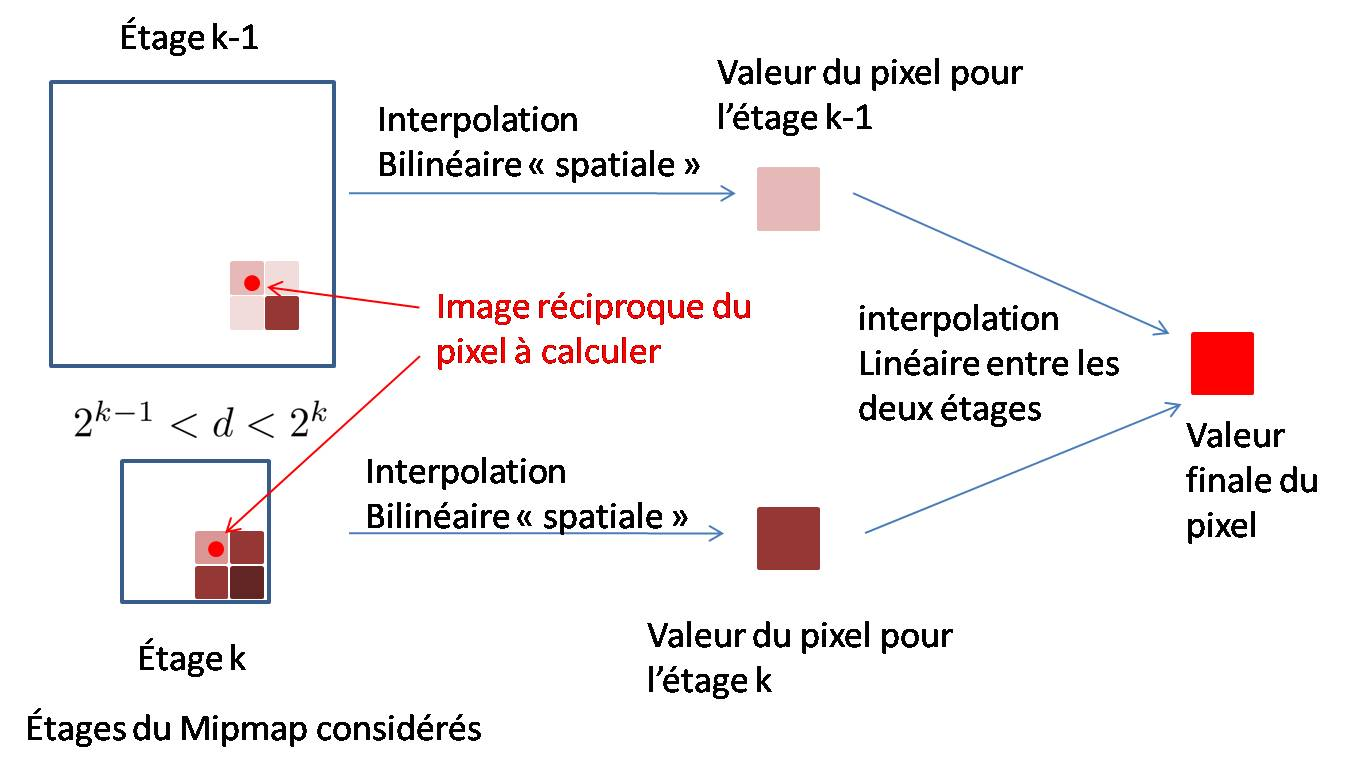
\includegraphics[scale=0.5]{intertrilineaire.jpg}
\end{figure}

\ssse{La fonction de distance}

Toutes les fonctions de distance proviennent de la différentielle de l'homographie inverse.
On note $(u,v)$ les coordonnées de l'image d'origine et $(x,y)$ celles dans la fenêtre d'arrivée.

Il est aisé de calculer les coefficients des dérivées partielles. On note $H$ l'homographie inverse.

%re image prgm, avec les dérivé partielle indiqués

L'enjeu est que si $d$ est trop grand, l'image est inutilement floutée (on parle d'over-blurring), et si $d$ est trop petit l'image est aliasée.

On a jugé de la performance des méthodes "à vue". On compte à terme l'évaluer sur des cosinus/sinus.

On note $\dd_{(x,y)} H$ la différentielle de $H$ en $(x,y)$.

On note $(u,v)=H(x,y)$.

\sssse{Méthode du déterminant}
$$D(x,y) = \sqrt{\det \txt{d}_{(x,y)} H}$$
En effet le déterminant est l'aire du parallélogramme, donc prendre un carré de coté la racine donne un carré de même aire.

Le résultat est relativement satisfaisant.

%schéma avec un ârallélogramme et le carré correspondant

\sssse{Méthode du plus grand côté}
$$ D(x,y) = \max \left(\sqrt{\left(\frac{\dr u}{\dr x}\right)^2 + \left(\frac{\dr v}{\dr x}\right)^2},\sqrt{\left(\frac{\dr u}{\dr y}\right)^2 + \left(\frac{\dr v}{\dr y}\right)^2}\right)$$
On prend le plus grand côté du parallélogramme comme côté du carré. Le résultat est bon. Cette formule viens d'un article de Heckbert \cite{heckbert1983texture}.

Ce résultat est satisfaisant.

%schéma avec un ârallélogramme et le carré correspondant

\sssse{Méthode des diagonales}
$$D(x,y) = \max \left( \sqrt{\left(\frac{\dr v}{\dr x}-\frac{\dr  u}{\dr  x}\right)^2+\left(\frac{\dr v}{\dr y}-\frac{\dr  u}{\dr y}\right)^2}, \sqrt{\left(\frac{\dr u}{\dr x}+\frac{\dr  v}{\dr  x}\right)^2+\left(\frac{\dr u}{\dr y}+\frac{\dr  v}{\dr  y}\right)^2} \right)$$
On prend la plus grande diagonale du parallélogramme. Ici l'image est trop flou.

%schéma avec un parallélogramme et le carré correspondant

\sssse{Méthode des valeurs singulières}

On peut décomposer toute matrice $A$ en trois matrices $A = PDQ^{-1}$ où $P$ et $Q$ sont orthogonales et $D$ est diagonale.

Pour cela on diagonalise $AA^t$, et $A^tA$, on prend $P$ et $Q$ des vecteurs propres normalisés de ces matrices, et $D$ la racine de leur diagonalisée. Il faut veiller à ce que $P$ et $Q$ correspondent bien \cite{abdi2007singular}.

Les coefficients de $D$ sont appelés valeurs singulières de $A$. On prend $D(x,y)$ le maximum des deux valeurs singulières de $A$.

Rq : On a une interprétation géométrique à l'aide d'une caméra de ces valeurs.

\sssse{Conclusion}

Les méthode du déterminant, du maximum des côtés et des valeurs singulières sont satisfaisantes.

On a une préférence pour le plus grand côté et la valeur singulière, en effet le déterminant semble introduire un peu plus d'aliasing. 

\ssse{Algorithme amélioré : Le ripmap}

Une des grandes faiblesses est l'anisotropie du mipmap : il ne privilégie aucune direction. Ainsi si le parallélogramme à approximer et en fait un rectangle très plat, il n'y a pas d'approximation raisonnable à l'aide d'un carré.

Pour tenter de palier à ce problème on utilise un ripmap \cite{akenine2008real}. C'est en fait un mipmap où l'on a aussi calculé la moyenne des pixels de tous les rectangles dont les côtés sont des puissances de deux.

Ainsi la fonction de distance ne renvoie plus une valeur mais deux, une pour chaque côté du rectangle. On réalise alors une interpolation bi-bi-linéaire (bilinéaire entre les niveaux et bilinéaire dans chacun d'eux).

%un vrai ripmap, que je ferais moi
\begin{figure}[h!]
\centering
\caption{Un exemple de Ripmap}
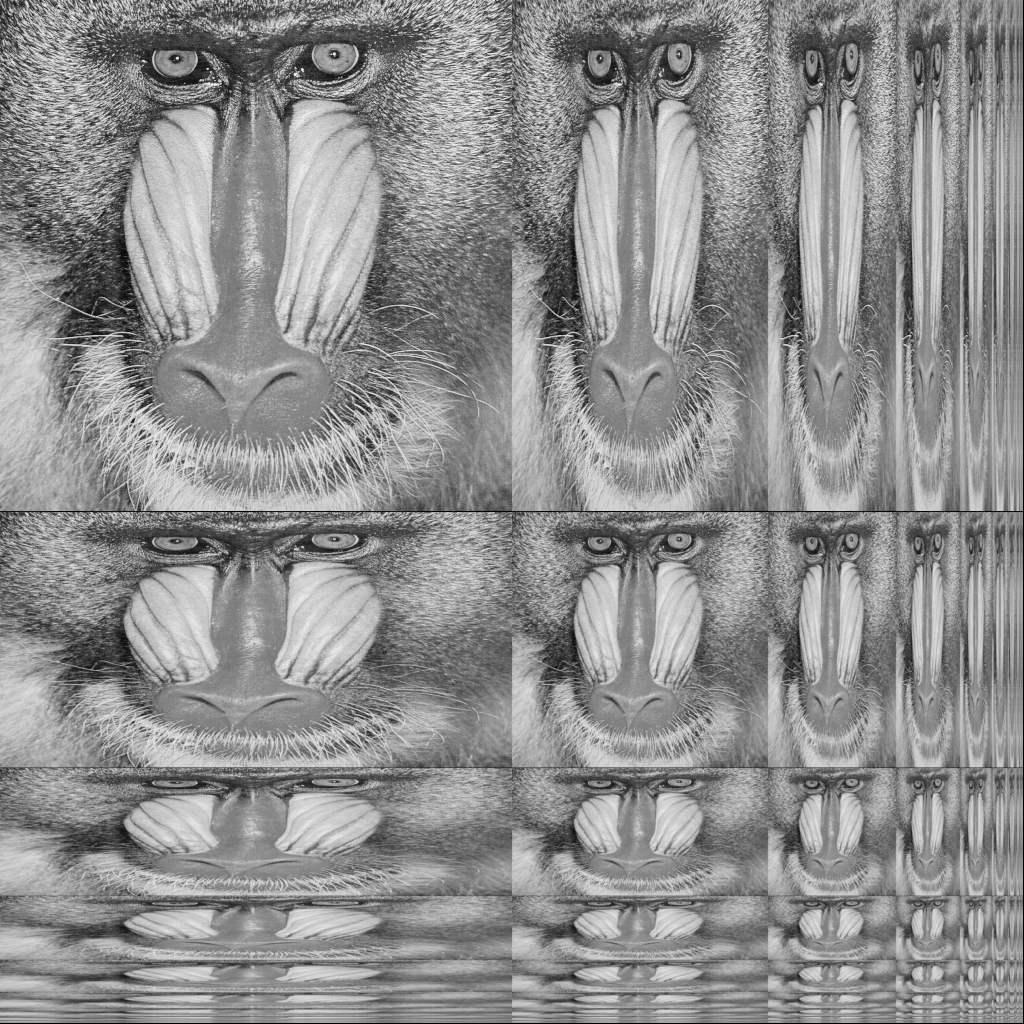
\includegraphics[scale=0.4]{Ripmap_real}
\end{figure}


%schéma d'interpolations pour le ripmap, avec 4 images est l'endroit ou le point tombe dans chacun
\begin{figure}[h!]
\centering
\caption{Schéma d'interpolation bi-bi-linéaire}
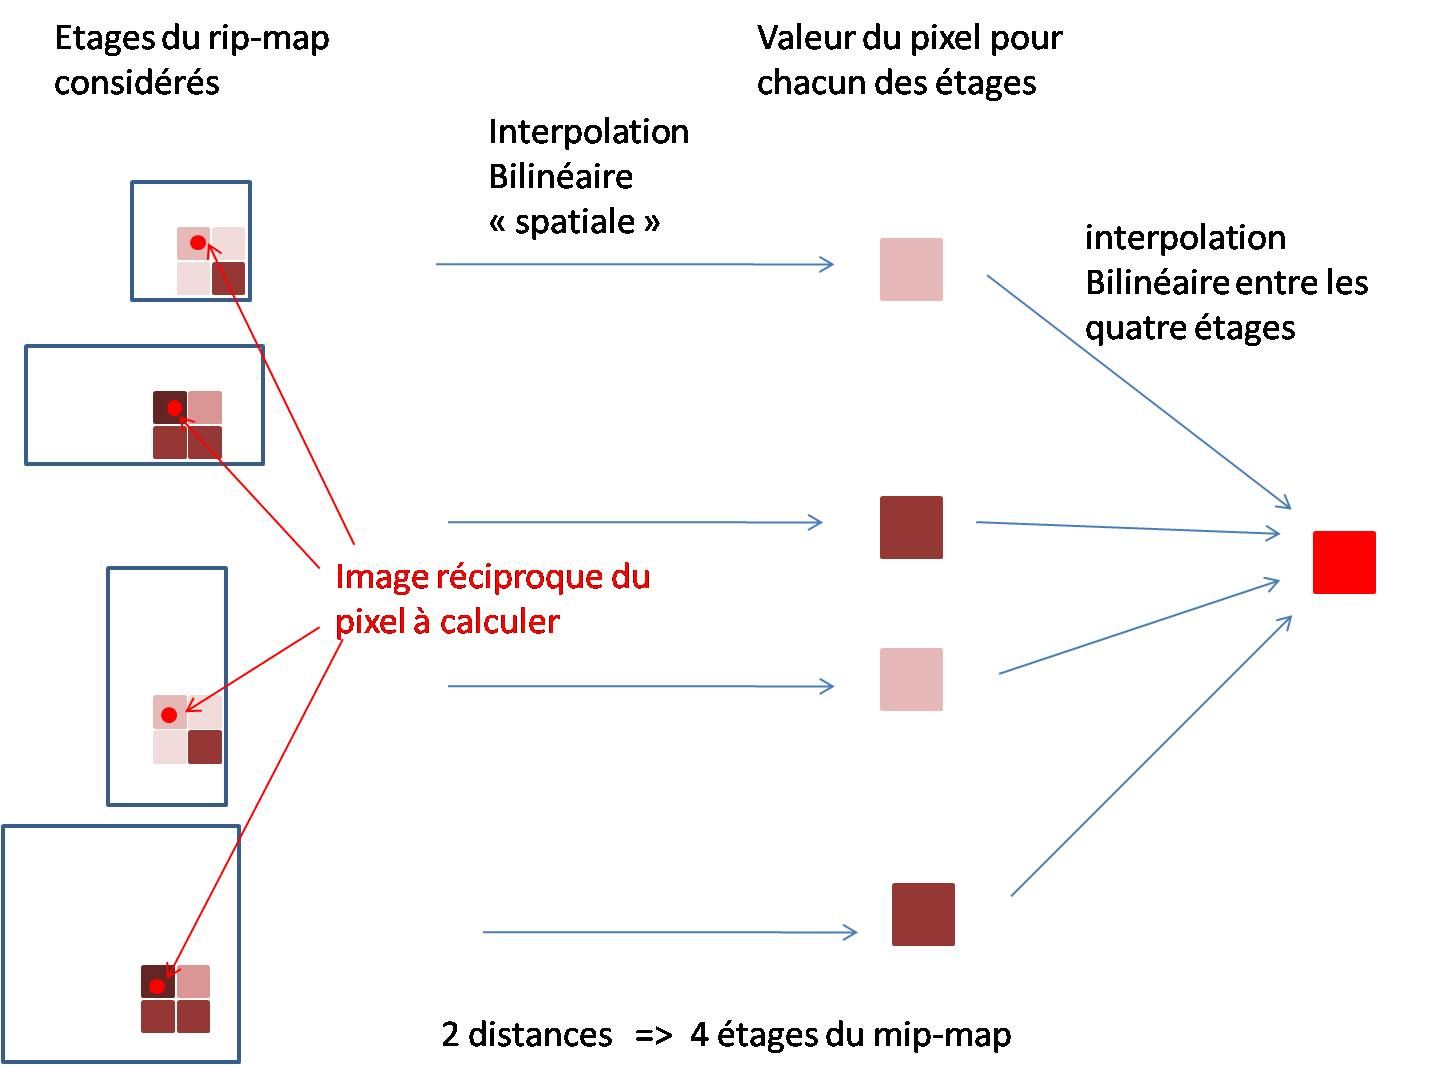
\includegraphics[scale=0.5]{interbibilineaire.jpg}
\end{figure}


On a utilisé le plus petit rectangle qui contient le parallélogramme. Ainsi la formule est de :
$$D(x,y) = \left( |\frac{\dr u}{\dr x}|+|\frac{\dr u}{\dr y}|,|\frac{\dr v}{\dr x}|+|\frac{\dr v}{\dr y}|\right)$$
On a de plus décalé les points pour que le rectangle considéré soit bien celui qui contient le parallélogramme.

Cela améliore certes la méthode, mais ne résous pas par exemple le cas d'un rectangle fin en diagonale.


